\RequirePackage{fix-cm}
\documentclass[smallcondensed]{svjour3}

\usepackage[T1]{fontenc}
\usepackage{newtxtext,newtxmath}
\usepackage{graphicx}
\usepackage{tabularx}
\usepackage{array}
\usepackage{amsmath}
\usepackage{microtype}
\usepackage{xurl}
\usepackage{placeins}
\usepackage[hidelinks]{hyperref}

\setlength{\emergencystretch}{2em}
\setlength{\textfloatsep}{10pt plus 2pt minus 2pt}
\setlength{\floatsep}{8pt plus 2pt minus 2pt}
\setlength{\intextsep}{9pt plus 2pt minus 2pt}
\renewcommand{\arraystretch}{1.14}
\setlength{\tabcolsep}{5pt}
\graphicspath{{figures/}}
\newcommand{\vect}[1]{\boldsymbol{#1}}
\newcommand{\tabnote}[1]{\vspace{2pt}\parbox{0.94\textwidth}{\footnotesize\textit{Note.} #1}}
\newcommand{\fignote}[1]{\vspace{2pt}\parbox{0.80\textwidth}{\footnotesize\textit{Note.} #1}}
\raggedbottom
\setcounter{topnumber}{4}
\setcounter{bottomnumber}{3}
\setcounter{totalnumber}{6}
\renewcommand{\topfraction}{0.92}
\renewcommand{\bottomfraction}{0.85}
\renewcommand{\textfraction}{0.08}
\renewcommand{\floatpagefraction}{0.80}
\journalname{International Journal of Intelligent Transportation Systems Research}

\begin{document}

\title{Reliability-Informed Traffic Speed Forecasting from Sparse Floating-Car Data on a Data-Scarce Highway Corridor}

\author{
Sun Wenjie\thanks{Corresponding author}
\and
Safizahanin binti Mokhtar
\and
Gabriel Ling Hoh Teck
\and
Li Ruiqing
\and
Liu Lvmin
}

\institute{
Sun Wenjie \at
Department of Urban and Regional Planning,
Universiti Teknologi Malaysia,
81310 Skudai, Johor, Malaysia \\
\email{sunwenjie@graduate.utm.my} \\
\emph{Corresponding author}
\and
Safizahanin binti Mokhtar \at
Department of Urban and Regional Planning,
Universiti Teknologi Malaysia,
81310 Skudai, Johor, Malaysia \\
\email{safizahanin@utm.my}
\and
Gabriel Ling Hoh Teck \at
Department of Urban and Regional Planning,
Universiti Teknologi Malaysia,
81310 Skudai, Johor, Malaysia \\
\email{gabriel.ling@utm.my}
\and
Li Ruiqing \at
Faculty of Computing,
Universiti Teknologi Malaysia,
81310 UTM Johor Bahru, Johor, Malaysia \\
\email{liruiqing@graduate.utm.my}
\and
Liu Lvmin \at
School of Information Engineering,
Nanjing Normal University Taizhou College,
Taizhou, Jiangsu Province, China \\
\email{lIml194568495@gmail.com}
}

\titlerunning{Sparse-FCD Traffic Speed Forecasting}
\authorrunning{Sun Wenjie et al.}

\maketitle

\begin{abstract}
Traffic speed forecasting supports route guidance and corridor control on highways with limited sensing. Most models are evaluated on dense sensor networks, so their validity with incomplete floating-car data (FCD) remains uncertain. Sparse FCD also produces uneven sample availability across locations and time. Future-data leakage and different test samples can distort model comparisons. This study examines the Pan Borneo Highway, a long interurban corridor in Sarawak, Malaysia. A 15-min FCD stream is cleaned, aligned to an hourly panel, and used to predict mean speed over 1-, 3-, and 6-h future windows. Seven models are evaluated on the same chronological samples. TCN ablation, stress tests, and regime analysis examine feature value and conditions associated with large errors. By fixing samples and preprocessing rules, the evaluation removes unequal-sample bias; XGBoost records the lowest MAEs of 0.9736, 0.8689, and 0.7867 km/h. Missing observations cause the largest error increase, while high-volatility and degraded traffic states remain the most difficult regimes. Future work should test longer records, other corridors, independent sensors, and calibrated prediction intervals.
\keywords{Floating-car data \and Traffic speed forecasting \and Sparse data \and Data reliability \and Highway corridor \and Intelligent transportation systems}
\end{abstract}

\section{Introduction}
Traffic speed forecasting supports route guidance, travel-time information, incident response, and highway operations. On long interurban roads, delayed action is costly because access points and diversion routes are limited. Short-window forecasts can help operators issue warnings before a disturbance spreads.

The Pan Borneo Highway in Sarawak, Malaysia, presents this problem in a data-scarce setting. The corridor connects dispersed communities and carries regional passenger and freight traffic. Fixed detectors are not available continuously along the route. Figure~\ref{fig:workflow} maps the 51 virtual FCD query points and outlines the forecasting process. Similar conditions occur on regional highways in Southeast Asia, where road expansion has outpaced sensor deployment.

Traffic forecasting studies have used recurrent, convolutional, graph-based, and attention-based models. Jiang and Luo reviewed graph neural networks for road-network dependence \cite{ref1}. Yu et al. applied an Autoformer to FCD-based traffic-state prediction \cite{ref4}. Yasuda et al. derived a network representation from trajectories, while Leinonen et al. used an LSTM with multiple data sources \cite{ref5,ref6}.

Sparse highway FCD creates three evaluation problems. Uneven provider coverage changes which samples are available. Scaling, imputation, target construction, and random splitting can introduce future information. Model-specific filtering can also create unequal test sets. Average error alone does not show whether missing observations, speed volatility, or degraded traffic causes the largest failures \cite{ref9,ref11}.

The study evaluates whether incomplete FCD can support controlled short-window forecasting on a long highway corridor. It asks how to form chronological samples without future leakage, which model performs best on the processed data, and where errors are concentrated. The contributions are an audited hourly panel, a future-window target, a seven-model comparison on shared samples, TCN stress tests, and regime-specific error analysis. No new neural architecture is proposed.

Section~2 reviews forecasting methods and the evaluation gap. Section~3 describes the corridor, data preparation, and chronological split. Section~4 defines the inputs, targets, reliability variables, leakage controls, and metrics. Section~5 gives the experimental protocol. Section~6 reports the results. Section~7 discusses the findings and limitations, and Section~8 concludes the paper.

\clearpage
\begin{figure}[!t]
\centering
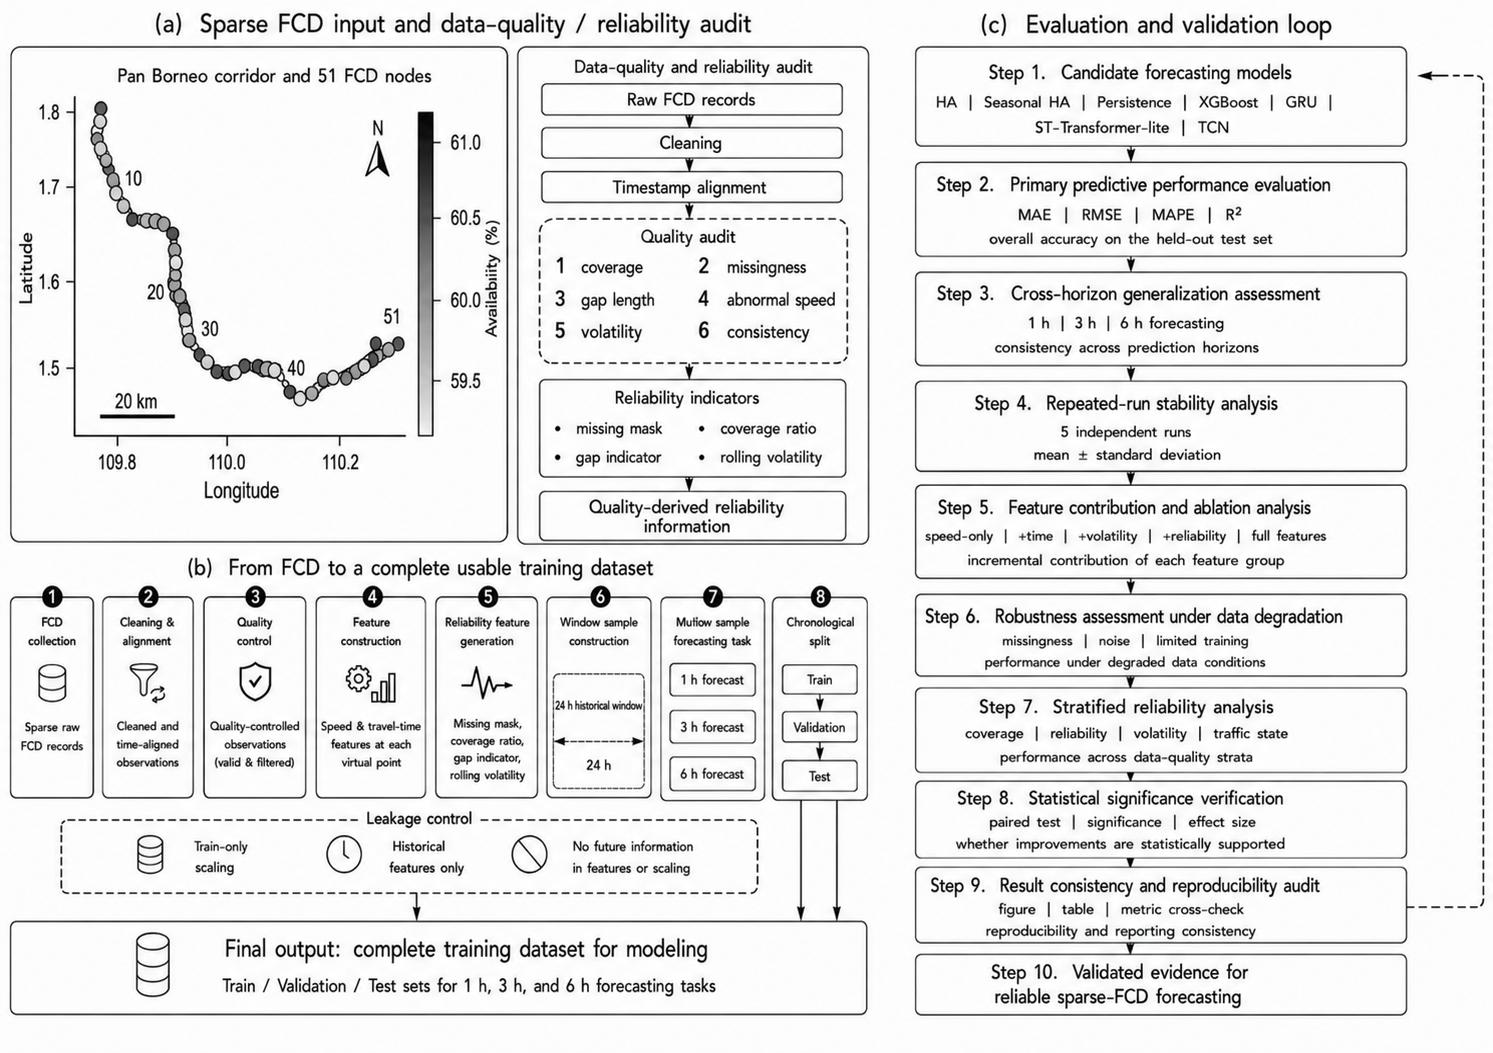
\includegraphics[width=0.74\textwidth]{fig1_corridor_workflow.png}
\caption{Pan Borneo study corridor and the sparse-FCD forecasting process.}\label{fig:workflow}
\fignote{The 51 mapped locations are virtual FCD query points. The process includes data cleaning, quality checks, leakage-controlled sample construction, model comparison, and regime analysis.}
\end{figure}
\FloatBarrier
\section{Related Work and Research Gap}
\subsection{Forecasting models and data representations}
Jiang and Luo explained how graph neural networks represent road topology in traffic forecasting \cite{ref1}. Ahmed et al. found that graph-based information fusion can improve prediction when several stable data channels are available \cite{ref2}. Yu et al. used an Autoformer to model long-range temporal patterns in FCD \cite{ref4}. These studies use structured datasets and do not establish which model class is most suitable for a short, incomplete highway record.

\subsection{Probe data and corridor forecasting}
Yasuda et al. constructed a traffic-network representation from vehicle trajectories and used it for deep traffic-state prediction \cite{ref5}. Leinonen et al. combined several data sources in an LSTM model and reported better prediction after adding those inputs \cite{ref6}. Zhang et al. noted that FCD quality depends on penetration, sampling, vehicle mix, and provider processing \cite{ref7}. These studies give limited detail on how irregular provider observations are converted into shared samples for model comparison.

\subsection{Missingness, reliability, and evaluation validity}
Zhang et al. distinguished random gaps, temporal blocks, and spatial patterns in missing traffic data \cite{ref9}. Torrisi et al. treated FCD penetration as a variable that changes across time and space \cite{ref8}. Mallick et al. used deep ensembles to quantify uncertainty in spatiotemporal traffic forecasts \cite{ref11}. These studies address missing data, FCD reliability, and uncertainty separately. They do not examine target eligibility, shared test samples, stress sensitivity, and regime-specific error within one sparse-corridor experiment.

\subsection{Research gap addressed in this study}
The remaining problem is how to compare forecasting models when observations are incomplete and provider-dependent. The evaluation uses explicit masks, future-window targets, chronological splits, shared point--time identifiers, repeated runs, TCN stress tests, and regime-specific error groups. These controls connect data quality with model evaluation and interpretation for corridor operation.
\section{Study Corridor and Data Preparation}
\subsection{Corridor and raw observations}
The study corridor is part of the Pan Borneo Highway in Sarawak, Malaysia. It represents a long interurban road with dispersed settlements, regional traffic, and limited fixed sensing. Such corridors require traffic monitoring without dense roadside detectors. Fifty-one virtual FCD points were placed along the route. They are provider query locations, not physical detectors.

The observation period covers 8 December 2025 to 28 February 2026. The 15-min records contain current speed, travel time, free-flow references, time, point identifier, and provider status. The theoretical panel contains 403,665 point--time slots. Valid observations account for 242,883 slots, giving 60.17\% coverage.

\subsection{Cleaning, hourly alignment, and split}
All timestamps were converted to one time standard. Records were sorted by point and time. Duplicate, invalid, and failed-status records were removed. The retained observations were then assigned to the analysis-ready hourly panel. The public release includes the hourly values and the fields \texttt{observed\_count}, \texttt{has\_observation}, and \texttt{missing\_mask}. Restricted provider responses are not redistributed.

The hourly panel contains 100,980 aligned rows, of which 97,094 are observed. Its coverage is 96.15\%. Hourly alignment reduces sub-hourly sparsity and supports 24-h histories, although it can smooth short disturbances. The chronological split contains 70,686 training rows, 15,147 validation rows, and 15,147 test rows. All transformations and feature statistics were fitted on the training period.

A sample was retained only when its input and target windows stayed within the same split and met the observation threshold. The shared test sets contain 12,265 samples at 1 h, 11,878 at 3 h, and 12,166 at 6 h. Every model used the same identifiers within each forecast window. Table~\ref{tab:data} summarises the data and task.
\begin{table}[!htbp]
\caption{Data source and forecasting task definition.}\label{tab:data}
\centering\small
\begin{tabularx}{0.94\textwidth}{>{\raggedright\arraybackslash}p{0.25\textwidth}X}
\hline
\textbf{Item} & \textbf{Definition}\\
\hline
Study setting & Pan Borneo Highway corridor, Sarawak, Malaysia; 51 virtual FCD points\\
\hline
Raw stream & 15-min observations, 8 Dec 2025--28 Feb 2026\\
\hline
Raw availability & 242,883 / 403,665 slots; 60.17\% coverage\\
\hline
Hourly analysis panel & Hourly; 97,094 / 100,980 rows observed; 96.15\% coverage\\
\hline
Chronological split & 70,686 train; 15,147 validation; 15,147 test rows\\
\hline
History and targets & 24-h history; future-window mean speed over 1-, 3-, and 6-h windows\\
\hline
Shared test samples & 12,265; 11,878; and 12,166 samples\\
\hline
\end{tabularx}
\tabnote{Counts are taken from the archived processed panel. The 51 FCD points are virtual provider-query locations rather than physical roadside detectors.}
\end{table}



\section{Reliability-Informed Forecasting Framework}
\subsection{Observed-data representation and historical input}
Let $i\in\{1,\ldots,N\}$ index the virtual FCD points and let $t$ index hourly time. The stored speed is $v_{i,t}$, and $m_{i,t}$ records whether that speed is observed \cite{ref7,ref9}:
\begin{equation}
m_{i,t}=
\begin{cases}
1, & \text{if a valid hourly speed is available at point }i\text{ and time }t,\\
0, & \text{otherwise.}
\end{cases}
\label{eq:mask}
\end{equation}
Here, $N=51$, $i$ is the point index, $t$ is the hourly index, and $m_{i,t}$ is dimensionless. The mask records availability and is not an imputed traffic value.

For a $P$-hour historical window ending at $t$, coverage is the share of observed slots and missingness is its complement \cite{ref8,ref9}:
\begin{equation}
\operatorname{cov}_{i,t}^{(P)}
=\frac{1}{P}\sum_{k=t-P+1}^{t}m_{i,k},
\qquad
\operatorname{miss}_{i,t}^{(P)}
=1-\operatorname{cov}_{i,t}^{(P)}.
\label{eq:coverage}
\end{equation}
In Eq.~\eqref{eq:coverage}, $k$ indexes the hours in the window and $P=24$. Both measures lie in $[0,1]$. The maximum gap is stored separately because two windows with equal coverage can contain different interruption patterns \cite{ref9}.

Traffic forecasting models use a historical sequence and optional contextual variables to estimate future speed \cite{ref1,ref3,ref4}. The input is
\begin{equation}
\vect{S}_{i,t}^{(P)}
=
[\vect{x}_{i,t-P+1},\ldots,\vect{x}_{i,t}],
\qquad P=24,
\label{eq:input}
\end{equation}
where $\vect{x}_{i,k}$ is the feature vector at point $i$ and hour $k$. The vector $\vect{z}_{i,t}$ contains time, coverage, maximum gap, volatility, and traffic-state descriptors. Each descriptor is computed no later than the forecast origin.

\subsection{Future-window target and model mapping}
The target is the mean observed speed during the next $h$ hours, rather than the speed only at $t+h$. This form represents traffic conditions over an operating window \cite{ref5,ref6}. The observed future indices and their count are
\begin{equation}
\mathcal{O}_{i,t}^{(h)}
=
\{r\in\{1,\ldots,h\}:m_{i,t+r}=1\},
\qquad
q_{i,t}^{(h)}=|\mathcal{O}_{i,t}^{(h)}|,
\label{eq:targetset}
\end{equation}
where $r$ is the lead-step index, $h\in\{1,3,6\}$ is the forecast-window length, and $q_{i,t}^{(h)}$ is the number of observed future hours. The target is
\begin{equation}
y_{i,t}^{(h)}
=
\frac{1}{q_{i,t}^{(h)}}
\sum_{r\in\mathcal{O}_{i,t}^{(h)}}v_{i,t+r}.
\label{eq:target}
\end{equation}
Here, $y_{i,t}^{(h)}$ is the future-window mean speed in km/h. Missing future speeds are excluded rather than imputed.

A sample is retained only when both the historical and future windows meet the preset observation threshold $\rho=0.80$:
\begin{equation}
\operatorname{cov}_{i,t}^{(P)}\geq\rho,
\qquad
\frac{q_{i,t}^{(h)}}{h}\geq\rho,
\qquad
\rho=0.80.
\label{eq:eligibility}
\end{equation}
The 1-h target requires the next hour. The 3-h target requires all three future hours, and the 6-h target requires at least five. Averaging smooths short-term variation, so lower error at a longer window does not mean that exact long-horizon prediction is easier \cite{ref6,ref19}.

For each forecast window, the model mapping is \cite{ref1,ref2,ref4}
\begin{equation}
\widehat{y}_{i,t}^{(h)}
=
F_h\!\left(\vect{S}_{i,t}^{(P)},\vect{z}_{i,t};\vect{\theta}_h\right),
\label{eq:model}
\end{equation}
where $\widehat{y}_{i,t}^{(h)}$ is the predicted future-window mean speed, $F_h$ is the forecast-window-specific model, and $\vect{\theta}_h$ contains its fitted parameters. All models within a forecast window use the same point, forecast-origin, and target identifiers.

\subsection{Volatility, leakage control, and candidate models}
A complete window can still be difficult when speed changes rapidly. Volatility is therefore measured separately from observation availability \cite{ref7,ref15}:
\begin{equation}
\operatorname{vol}_{i,t}^{(P)}
=
\frac{1}{|\mathcal{A}_{i,t}^{(P)}|}
\sum_{k\in\mathcal{A}_{i,t}^{(P)}}|v_{i,k}-v_{i,k-1}|,
\quad
\mathcal{A}_{i,t}^{(P)}
=
\{k:m_{i,k}=m_{i,k-1}=1\}.
\label{eq:volatility}
\end{equation}
The set $\mathcal{A}_{i,t}^{(P)}$ contains valid adjacent pairs in the $P$-hour window, and $\operatorname{vol}_{i,t}^{(P)}$ is measured in km/h per hourly transition.

Five controls limit leakage: chronological splitting, train-only scaling, historical-only features, fixed forecast-window masks, and stored point--time identifiers \cite{ref3,ref9}. The benchmark includes historical average, seasonal historical average, persistence, XGBoost, GRU, TCN, and ST-Transformer-lite. All models are compared under the same data, sample, and evaluation controls. No neural model is presented as the proposed method.

\subsection{Evaluation and effect measures}
Let $\Omega_h$ be the shared test set for forecast window $h$, with $M_h=|\Omega_h|$. MAE is the primary metric because it retains km/h. RMSE gives more weight to large errors, while sMAPE provides a scale-normalised measure \cite{ref18,ref19}:
\begin{equation}
\begin{aligned}
\operatorname{MAE}_h
&=\frac{1}{M_h}\sum_{(i,t)\in\Omega_h}|y_{i,t}^{(h)}-\widehat{y}_{i,t}^{(h)}|,\\
\operatorname{RMSE}_h
&=\sqrt{\frac{1}{M_h}\sum_{(i,t)\in\Omega_h}(y_{i,t}^{(h)}-\widehat{y}_{i,t}^{(h)})^2},\\
\operatorname{sMAPE}_h
&=\frac{100}{M_h}\sum_{(i,t)\in\Omega_h}
\frac{2|y_{i,t}^{(h)}-\widehat{y}_{i,t}^{(h)}|}
{|y_{i,t}^{(h)}|+|\widehat{y}_{i,t}^{(h)}|+\varepsilon}.
\end{aligned}
\label{eq:metrics}
\end{equation}
In Eq.~\eqref{eq:metrics}, $\varepsilon>0$ is a fixed numerical safeguard applied identically to all models.

Ablation and stress-test effects use a fixed reference. Model comparisons use paired absolute errors on the same samples \cite{ref17,ref20,ref21}:
\begin{equation}
\begin{aligned}
\Delta\operatorname{MAE}(\%)
&=
100\,
\frac{\operatorname{MAE}_{\mathrm{condition}}-\operatorname{MAE}_{\mathrm{reference}}}
{\operatorname{MAE}_{\mathrm{reference}}},\\
d_{i,t}^{(h)}
&=
|y_{i,t}^{(h)}-\widehat{y}_{i,t,\mathrm{candidate}}^{(h)}|
-
|y_{i,t}^{(h)}-\widehat{y}_{i,t,\mathrm{reference}}^{(h)}|.
\end{aligned}
\label{eq:effects}
\end{equation}
Positive values indicate degradation or a larger candidate error. Seed-level comparisons use the Wilcoxon signed-rank test with Holm correction. Because only five seed pairs are available, interpretation focuses on effect size and direction rather than statistical significance.
\section{Experimental Design}
\subsection{Training protocol and configurations}
Experiments were run in Python 3.10 with CUDA-enabled PyTorch on an NVIDIA RTX A3000 Laptop GPU. Short diagnostic runs checked data loading, tensor dimensions, masks, and output files. Only full runs are reported. Neural models were trained for at most 30 epochs. Validation MAE selected the checkpoint, and training stopped after five epochs without improvement. The learning rate was 0.001, weight decay was 0.0001, and the gradient norm was limited to 1.0.

Table~\ref{tab:models} lists the main configurations. The set includes transparent baselines, a tree-based model, recurrent and convolutional networks, and a lightweight Transformer. This range tests whether added model complexity is useful for the three-month hourly record. Full configurations, checkpoints, seed-level outputs, and environment records are stored in the public package.
\begin{table}[!htbp]
\caption{Candidate models and principal configurations.}\label{tab:models}
\centering\scriptsize
\begin{tabularx}{0.94\textwidth}{>{\raggedright\arraybackslash}p{0.20\textwidth}>{\raggedright\arraybackslash}p{0.27\textwidth}X}
\hline
\textbf{Model} & \textbf{Representation} & \textbf{Principal setting}\\
\hline
HA & Historical speed & Training-history mean\\
\hline
SeasonalHA & Speed and time index & Hour/seasonal mean\\
\hline
Persistence & Latest observed speed & No fitted parameters\\
\hline
XGBoost & Tabular lags and descriptors & 500 trees; depth 8; learning rate 0.05; subsample 0.8\\
\hline
GRU & Historical sequence & Hidden size 64; one layer\\
\hline
TCN & Historical sequence & Channels 32/32/32; kernel 3; dropout 0.1\\
\hline
ST-Transformer-lite & Historical sequence & $d_{\mathrm{model}}=32$; 4 heads; 2 layers; feed-forward size 64\\
\hline
\end{tabularx}
\tabnote{Only the principal settings used to interpret the comparison are shown. Complete configurations, seeds, checkpoints, and environment records are archived with the reproducibility package.}
\end{table}

\subsection{Benchmark, ablation, stress tests, and statistical analysis}
The benchmark includes seven models and three forecast windows. Stochastic models used five seeds, while deterministic baselines were evaluated once. Model selection used the validation period. Final results were calculated on the held-out test period.

The TCN ablation used the same split, seeds, and masks. It compared speed only, speed with time, speed with volatility, speed with reliability variables, and the full feature set. TCN was also used for the stress tests. Added missingness was set to 0\%, 10\%, 20\%, or 30\%. Noise was tested at four levels, and the retained training ratios were 20\%, 40\%, 60\%, 80\%, and 100\%. Missingness and noise affected only historical inputs. Targets, validation samples, and test samples were unchanged.

The five seeds were 42, 2024, 2025, 2026, and 3407. Each perturbed condition was paired with the clean or full-training result for the same seed. Supplementary outputs report Wilcoxon signed-rank tests, Holm-adjusted values, and rank-biserial effect sizes \cite{ref20,ref21}. None of the stress-test comparisons remained significant after correction. The results describe TCN sensitivity and do not establish the behaviour of all models.
\section{Results}
\subsection{Main forecasting performance and model stability}
XGBoost had the lowest MAE at all three forecast windows. Its MAE was $0.9736\pm0.0080$ km/h at 1 h, $0.8689\pm0.0059$ km/h at 3 h, and $0.7867\pm0.0028$ km/h at 6 h (Table~\ref{tab:main}). The largest standard deviation was 0.0080 km/h. This small variation supports a stable ranking across runs. The hourly FCD panel supports stable short-window prediction within the study period, but the results do not establish field deployment accuracy.

XGBoost reduced MAE by 15.22\%, 14.48\%, and 13.59\% relative to SeasonalHA. Relative to persistence, the reductions were 7.22\%, 33.71\%, and 50.91\%. The widening gap shows that the latest speed becomes less useful as the future window grows. SeasonalHA remained competitive at 3 h and 6 h, making it a useful fallback.

Figure~\ref{fig:benchmark}(a) places XGBoost at the lower edge of the model distributions. ST-Transformer-lite ranked second at 3 h and 6 h. GRU was closer to XGBoost at 1 h but weakened at the longer windows. Figure~\ref{fig:benchmark}(b) compares absolute errors on identical point--time samples. Most differences are positive, so the ranking is not caused by an easier test set for XGBoost.

The lower 6-h MAE reflects the target in Eq.~\eqref{eq:target}. The 3-h and 6-h targets average several future speeds and remove some short-term variation. They describe mean traffic conditions, not exact terminal speeds.

\begin{table}[!htbp]
\caption{Held-out mean absolute error across the three future-speed windows.}\label{tab:main}
\centering\scriptsize
\begin{tabular}{lcccc}
\hline
\textbf{Model} & \textbf{1 h} & \textbf{3 h} & \textbf{6 h} & \textbf{Rank 1/3/6 h}\\
\hline
XGBoost & $0.9736\pm0.0080$ & $0.8689\pm0.0059$ & $0.7867\pm0.0028$ & 1/1/1\\
\hline
ST-Transformer-lite & $1.0667\pm0.0556$ & $0.9847\pm0.0375$ & $0.9013\pm0.0223$ & 4/2/2\\
\hline
TCN & $1.1420\pm0.0878$ & $1.0113\pm0.0394$ & $0.9378\pm0.0173$ & 5/3/4\\
\hline
GRU & $1.0486\pm0.0378$ & $1.0337\pm0.0275$ & $0.9525\pm0.0506$ & 2/5/5\\
\hline
SeasonalHA & 1.1484 & 1.0160 & 0.9104 & 6/4/3\\
\hline
Persistence & 1.0494 & 1.3107 & 1.6026 & 3/6/7\\
\hline
HA & 1.9087 & 1.7670 & 1.5559 & 7/7/6\\
\hline
\end{tabular}
\tabnote{Values are mean $\pm$ standard deviation across five runs for stochastic models. Deterministic baselines are reported once. Models within a horizon use the same test identifiers.}
\end{table}

\begin{figure}[!htbp]
\centering
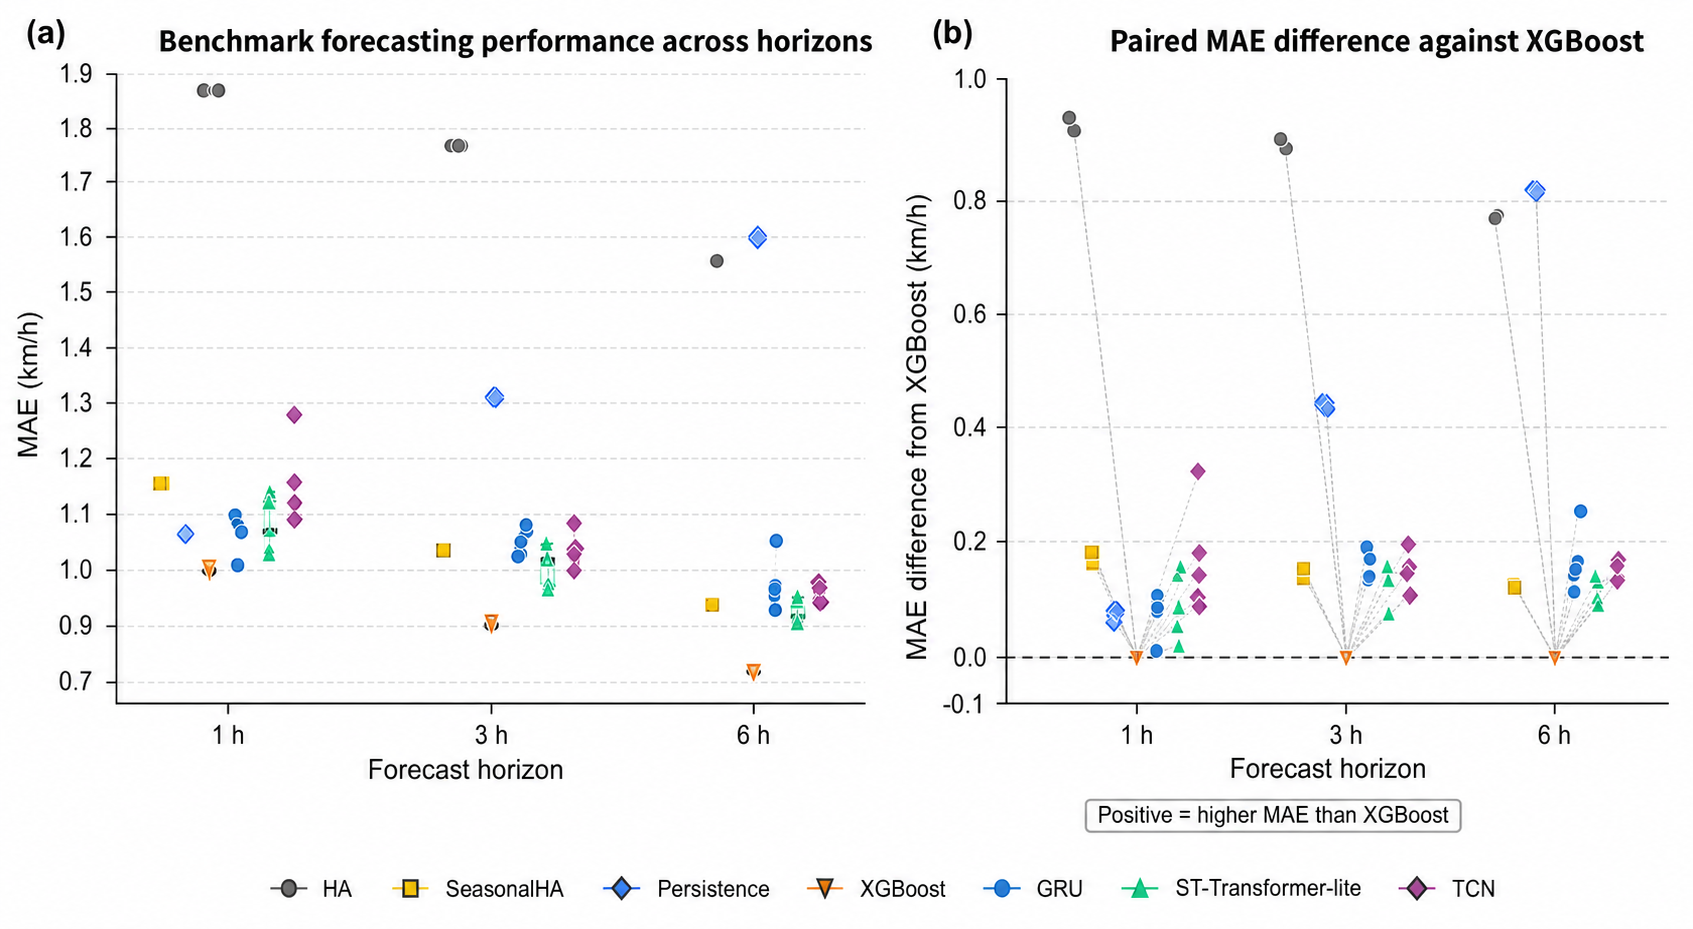
\includegraphics[width=0.76\textwidth]{fig2_main_benchmark.png}
\caption{Benchmark performance and paired absolute-error differences from XGBoost.}\label{fig:benchmark}
\fignote{Panel (a) compares MAE across horizons. Panel (b) subtracts XGBoost absolute error from each candidate's error on matched samples; positive values indicate a larger error than XGBoost.}
\end{figure}

\subsection{Feature contribution and reliability variables}
The ablation distinguishes the predictive use of reliability variables from their diagnostic use. Adding these variables to TCN did not consistently reduce error (Fig.~\ref{fig:ablation}). The full feature set was not the best configuration at any window.

Relative to speed only, the full feature set increased MAE by 26.69\%, 10.23\%, and 16.23\% at 1 h, 3 h, and 6 h. Adding volatility reduced 3-h MAE by 2.71\% but worsened the other two results. The effect therefore depends on the forecast window. With a short record, extra variables can add noise as well as useful information.

The reliability measures still serve two functions. Coverage and gap determine sample eligibility, and the same variables support warnings and error grouping. Their diagnostic role should not be presented as a general accuracy gain.

\begin{figure}[!htbp]
\centering
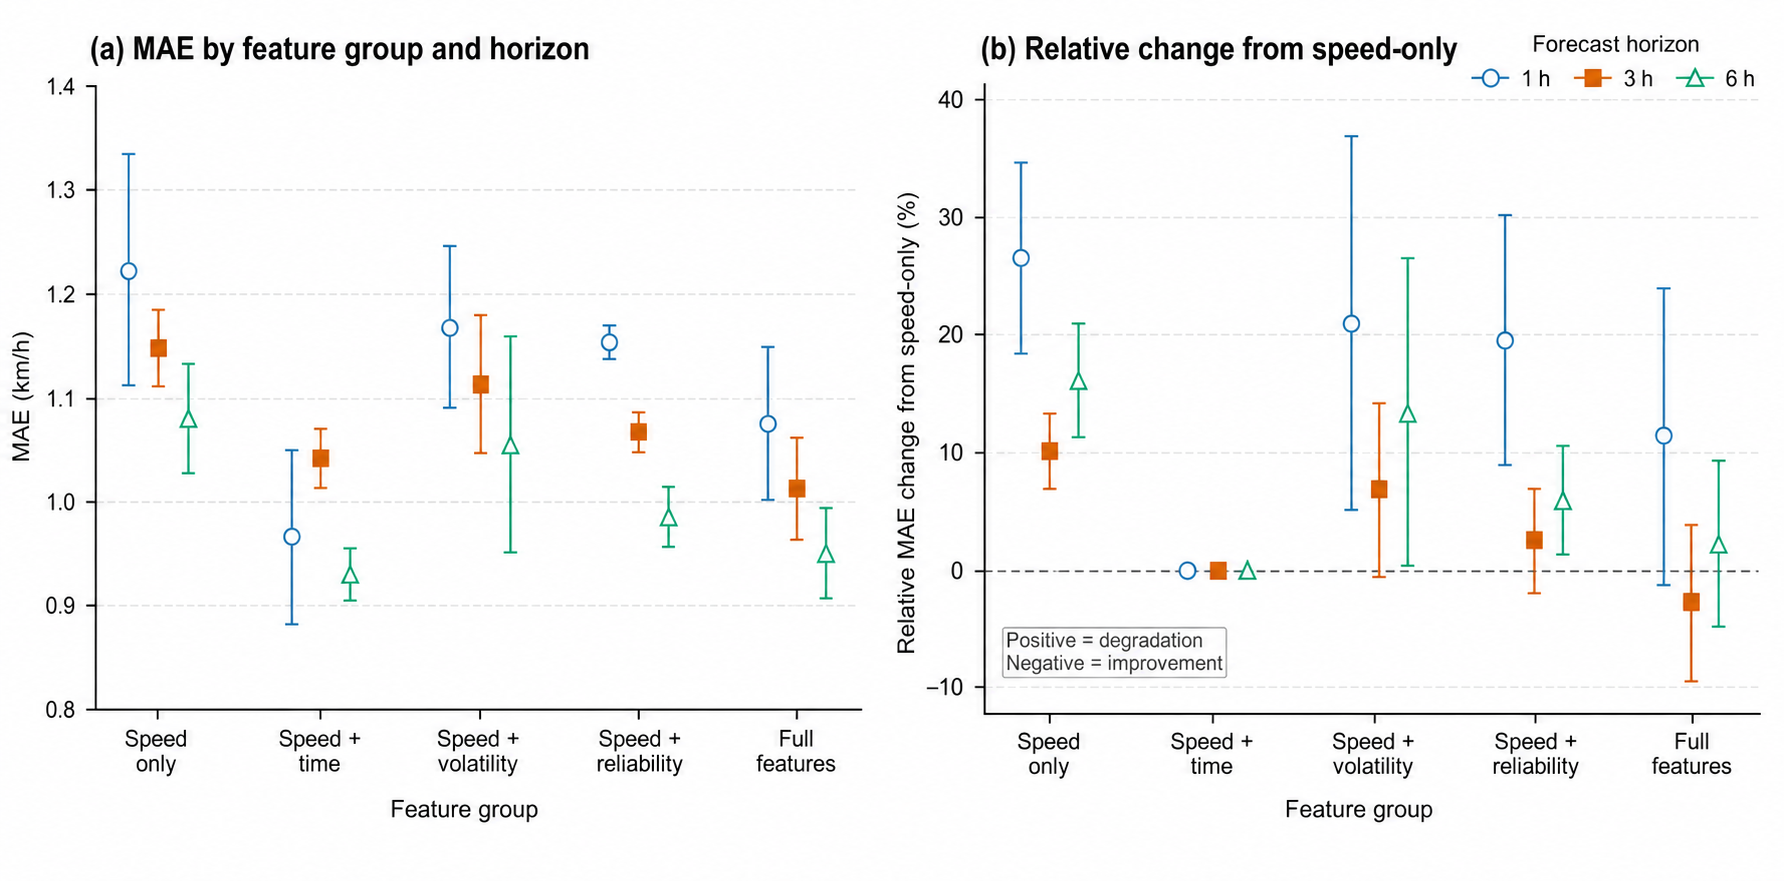
\includegraphics[width=0.76\textwidth]{fig3_ablation.png}
\caption{TCN feature-group ablation across forecast windows.}\label{fig:ablation}
\fignote{Panel (a) reports MAE by feature group and horizon. Panel (b) reports change from the TCN speed-only setting; positive values indicate degradation and negative values indicate improvement.}
\end{figure}

\subsection{Sensitivity to missingness, noise, and limited training data}
Historical missingness caused the largest accuracy loss in the TCN stress tests (Fig.~\ref{fig:robust}). At 30\% added missingness, the maximum relative MAE increase reached 268.0\%, 331.9\%, and 339.9\% at 1 h, 3 h, and 6 h. The larger increases at 3 h and 6 h show that incomplete histories remove information needed to describe a longer future interval.

Value noise had a smaller effect. At the highest level, the maximum increases were 26.4\%, 21.3\%, and 18.1\%. Noise changes recorded values but usually preserves their positions in time. Missingness removes parts of the sequence, which explains the larger deterioration.

Using only 20\% of the training data also increased MAE. Figure~\ref{fig:robust}(d) places this change well below the missingness effect. For the tested TCN, continuity in the recent input window mattered more than retaining every training sample.

The seed-level tests were not significant after Holm correction. These values are sensitivity estimates for TCN, not universal robustness results. A corridor system should monitor recent observation continuity and activate a warning or fallback when missingness rises.

\begin{figure}[!htbp]
\centering
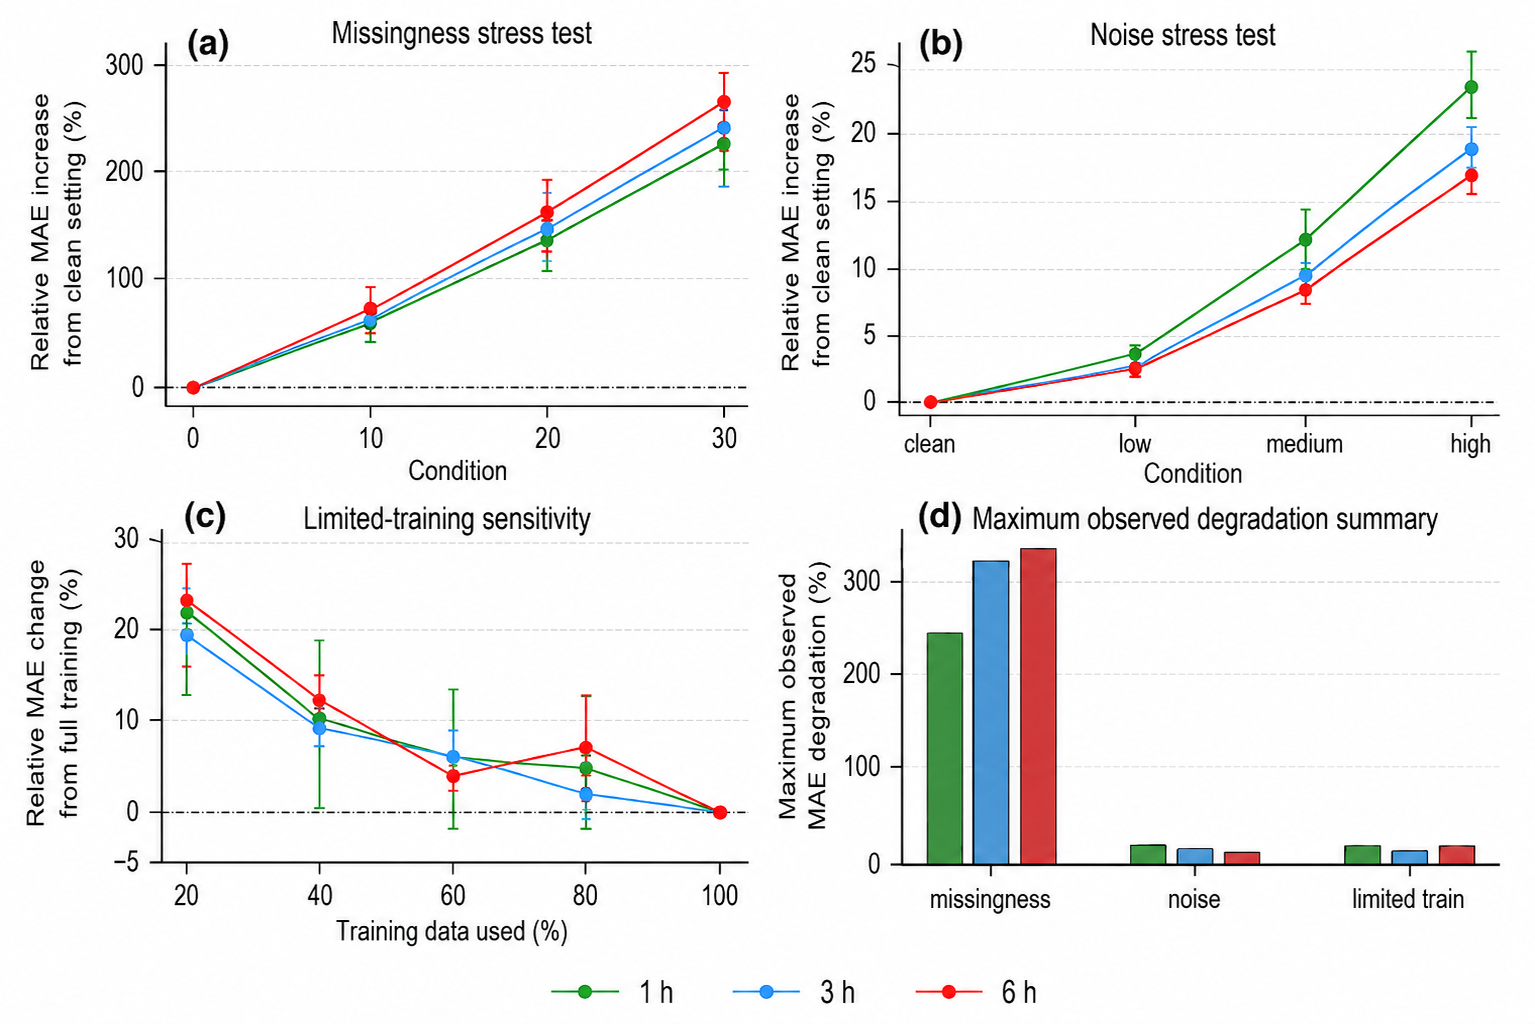
\includegraphics[width=0.72\textwidth]{fig4_robustness.png}
\caption{TCN sensitivity under missingness, value noise, and reduced training data.}\label{fig:robust}
\fignote{Missingness and noise affect only historical inputs; targets and test samples remain unchanged. Panels (a)--(c) show each stress condition, and panel (d) compares the largest degradation.}
\end{figure}

\subsection{Traffic regimes that concentrate error}
High volatility and degraded traffic were the most difficult regimes (Fig.~\ref{fig:regimes}). High-volatility MAE was 1.71, 1.53, and 1.40 km/h at 1 h, 3 h, and 6 h. These values were about 156\%, 156\%, and 150\% above the low-volatility reference. Rapid speed changes therefore remain difficult across all windows.

For degraded traffic, MAE was about 1.51, 1.53, and 1.49 km/h. The relative gaps were about 96\%, 126\%, and 164\%. The absolute error changed little, but the gap from the reference group increased with the forecast window. A warning should account for both recent speed instability and the current traffic state.

Coverage and reliability groups were not monotonic. Some high-coverage groups had larger errors than medium groups. Complete observations can occur during unstable or congested periods. Coverage alone is not enough to judge forecast difficulty. A corridor display should combine availability, gap length, volatility, traffic state, and forecast window.

\begin{figure}[!htbp]
\centering
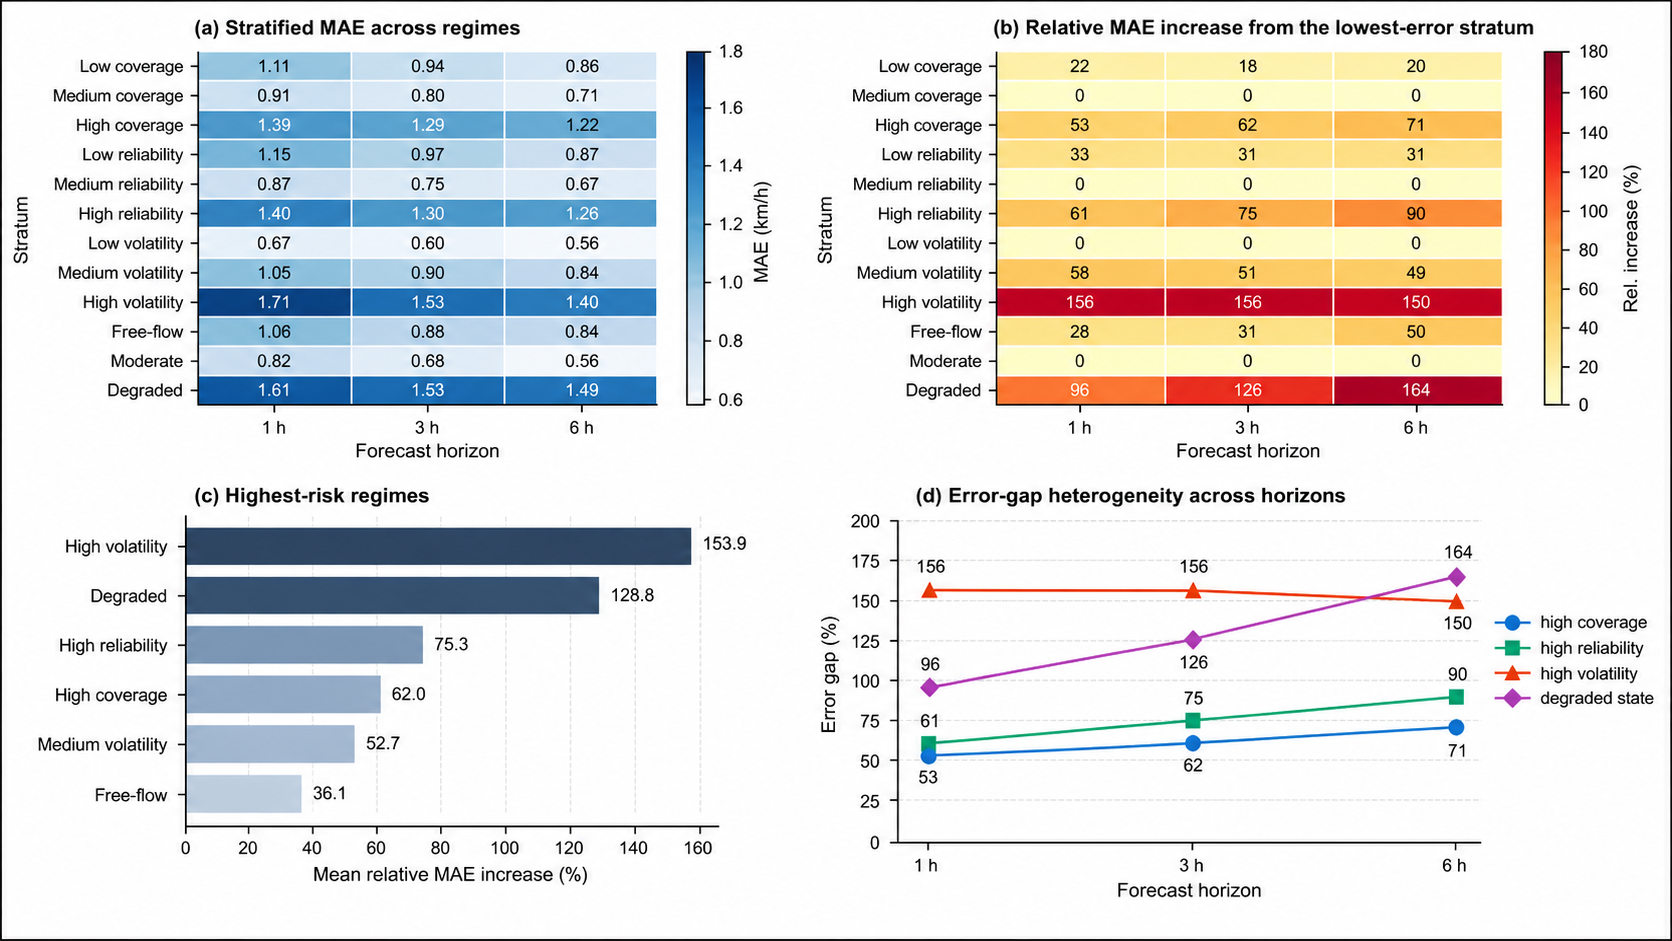
\includegraphics[width=0.76\textwidth]{fig5_regimes.png}
\caption{Forecast-error concentration across data-quality and traffic-state regimes.}\label{fig:regimes}
\fignote{Relative changes use the lowest-error stratum in each group as the reference. Supplementary files report the sample count for each stratum.}
\end{figure}

\subsection{Experimental usability and reproducibility}
The released hourly panel and common test sets support repetition from the processed-data stage onward. The audit retained 242,883 valid observations from 403,665 theoretical 15-min slots. Hourly alignment produced 97,094 observed rows from 100,980 possible rows, or 96.15\% coverage. The panel supports 24-h histories while retaining explicit missing-data indicators.

The common test sets contain 12,265, 11,878, and 12,166 samples at 1 h, 3 h, and 6 h. All models use the same forecast origins and targets. The benchmark identifies the best model on those samples. The ablation tests feature value, the stress tests measure sensitivity, and the regime analysis identifies difficult conditions.

Chronological splits, train-only transformations, common identifiers, five seeds, prediction files, and archived settings support replication. The GitHub commit and Zenodo record identify the analysed version. The study does not establish real-time deployment because raw acquisition and independent sensor validation are outside the released experiment. The reported analysis can nevertheless be audited and reproduced.

\FloatBarrier
\section{Discussion}
Yasuda et al. derived a network representation from vehicle trajectories, while Leinonen et al. combined several data sources in an LSTM model \cite{ref5,ref6}. The present analysis focuses on an earlier step: converting incomplete provider observations into valid, shared forecasting samples. The observation mask, target rule, and shared identifiers make each comparison traceable.

Jiang and Luo emphasized graph structure, and Ahmed et al. reported gains from information fusion when stable data channels are available \cite{ref1,ref2}. The XGBoost result is compatible with those findings. The present record covers three months, uses virtual query points, and contains limited topology. Under these data conditions, the tree-based model used the available lag and diagnostic variables more effectively than the tested sequence models. A more complex model should be retained only when it improves results on the same samples.

Zhang et al. showed that missing-data patterns affect the choice of reconstruction method \cite{ref9}. Torrisi et al. treated FCD penetration as a variable that changes over time and space \cite{ref8}. The TCN stress test applies these points to prediction. Added missingness removed temporal information and caused much larger errors than value noise. Observation continuity and gap length should be monitored during operation.

Mallick et al. argued that point predictions should be accompanied by uncertainty information \cite{ref11}. The regime results provide a related diagnostic by locating the largest errors in high-volatility and degraded traffic states. They do not replace calibrated prediction intervals. They identify conditions in which an operator may lower confidence, display a warning, or use a seasonal fallback.

The study is limited to one corridor, one provider, and a three-month period. The targets are derived from held-out FCD rather than independent fixed sensors. Hourly alignment can smooth short disturbances. The stress tests do not reproduce every incident, weather event, closure, or provider failure. The public archive begins with the processed hourly panel and excludes restricted raw responses. Longer records, independent sensors, external events, and additional corridors are needed before the model ranking and warning thresholds can be generalized.
\section{Conclusion}
Incomplete FCD supported repeatable short-window traffic forecasting on the Pan Borneo Highway when data quality, sample eligibility, and model comparison were controlled. XGBoost had the lowest MAE at the 1-h, 3-h, and 6-h windows. Reliability and volatility variables did not consistently improve TCN accuracy. Missing historical observations caused the largest stress-test degradation, while high volatility and degraded traffic produced the largest regime errors.

The findings extend beyond the model ranking. Sparse-corridor forecasts should also report observation quality, common-sample validation, and traffic-regime information. The released panel, fixed splits, stored identifiers, and archived outputs make the analysis reproducible from the processed-data stage. Longer records, independent measurements, other Southeast Asian corridors, external events, and calibrated prediction intervals are required before operational thresholds are set.
\section*{Statements and Declarations}
\noindent\textbf{Data availability:} Processed and anonymized data products, figure and table source files, configurations, statistical outputs, validation reports, and checksums are available at \url{https://github.com/tasadapullo-svg/2026-PanBorneo-FCD-Forecasting-Reproducibility}. The manuscript snapshot is \nolinkurl{conference_paper_support_package_20260706}, and the audited repository state is identified by commit \nolinkurl{aae70805623e63d82d77187d859919283d289062}. The associated Zenodo record is \url{https://doi.org/10.5281/zenodo.20901687}. Raw provider-level FCD records, API responses, credentials, and other restricted materials are not redistributed because of licensing and security constraints.\par

\noindent\textbf{Code availability:} Scripts for training, evaluation, statistical analysis, validation, and figure generation are included in the archived reproducibility package. The public materials support auditing from the processed hourly panel onward; complete reconstruction of provider-restricted raw acquisition requires independent authorized access.\par

\noindent\textbf{Funding:} The authors received no specific funding for this work.\par

\noindent\textbf{Competing interests:} The authors have no relevant financial or non-financial interests to disclose.\par

\noindent\textbf{Acknowledgements:} The authors thank the Faculty of Built Environment and Surveying, Universiti Teknologi Malaysia, for providing the laboratory environment and related support for system deployment and experimental operation. The authors also acknowledge the contextual information on corridor operation and transport planning in Sarawak, Malaysia. No individual or institution influenced the study design, data analysis, interpretation of results, or manuscript conclusions.\par

\begin{thebibliography}{99}
\bibitem{ref1} Jiang W, Luo J (2022) Graph neural network for traffic forecasting: a survey. Expert Syst Appl 207:117921. \url{https://doi.org/10.1016/j.eswa.2022.117921}
\bibitem{ref4} Yu S, Peng J, Ge Y, Ding F, Li S, Ma C (2024) A traffic state prediction method based on spatial-temporal data mining of floating car data by using Autoformer architecture. Comput-Aided Civ Infrastruct Eng. \url{https://doi.org/10.1111/mice.13179}
\bibitem{ref5} Yasuda S, Katayama H, Nakanishi W, Iryo T (2024) Trajectory data-driven network representation for traffic state prediction using deep learning. Int J Intell Transp Syst Res 22:136--145. \url{https://doi.org/10.1007/s13177-023-00383-z}
\bibitem{ref6} Leinonen M, Al-Tachmeesschi A, Turkmen B, Atashi N, Ruotsalainen L (2025) Long short term memory based traffic prediction using multi-source data. Int J Intell Transp Syst Res 23:354--371. \url{https://doi.org/10.1007/s13177-024-00451-y}
\bibitem{ref9} Zhang Y, Kong X, Zhou W, Liu J, Fu Y, Shen G (2024) A comprehensive survey on traffic missing data imputation. IEEE Trans Intell Transp Syst 25(12):19252--19275. \url{https://doi.org/10.1109/TITS.2024.3478816}
\bibitem{ref11} Mallick T, Macfarlane J, Balaprakash P (2024) Uncertainty quantification for traffic forecasting using deep-ensemble-based spatiotemporal graph neural networks. IEEE Trans Intell Transp Syst 25(8):9141--9152. \url{https://doi.org/10.1109/TITS.2024.3381099}
\bibitem{ref2} Ahmed SF, Kuldeep SA, Rafa SJ, Fazal J, Hoque M, Liu G, Gandomi AH (2024) Enhancement of traffic forecasting through graph neural network-based information fusion techniques. Inf Fusion 108:102466. \url{https://doi.org/10.1016/j.inffus.2024.102466}
\bibitem{ref7} Zhang C, Zhou Y, Zhang M, Wang B, Nie Y (2025) Review and prospect of floating car data research in transportation. J Traffic Transp Eng Engl Ed 12(4):752--771. \url{https://doi.org/10.1016/j.jtte.2024.09.005}
\bibitem{ref8} Torrisi V, Calabro G, De Souza Oliveira T, Inturri G, Cavalieri S, Ignaccolo M (2026) Exploring the reliability of floating car data through penetration rate prediction in urban contexts. Res Transp Bus Manag 64:101565. \url{https://doi.org/10.1016/j.rtbm.2025.101565}
\bibitem{ref3} Du K, Guo X, Li L, Song J, Shi Q, Hu M, Fang J (2025) Traffic prediction in time series, spatial-temporal, and OD data: a systematic survey. J Traffic Transp Eng Engl Ed. \url{https://doi.org/10.1016/j.jtte.2025.03.001}
\bibitem{ref19} Hyndman RJ, Koehler AB (2006) Another look at measures of forecast accuracy. Int J Forecast 22(4):679--688. \url{https://doi.org/10.1016/j.ijforecast.2006.03.001}
\bibitem{ref15} Ipekyuz B, Karatas Sevinen P, Tuydes Yaman H (2025) Performance evaluation of fused floating car data and Bluetooth data speed estimation on urban arterials. Arab J Sci Eng 50:17091--17108. \url{https://doi.org/10.1007/s13369-025-10088-y}
\bibitem{ref18} Hodson TO (2022) Root-mean-square error (RMSE) or mean absolute error (MAE): when to use them or not. Geosci Model Dev 15:5481--5487. \url{https://doi.org/10.5194/gmd-15-5481-2022}
\bibitem{ref17} Bai Y, Meng W, Gong Y, Li Y (2025) Advanced real-time highway risk early warning system integrating comprehensive weighting techniques. Int J Intell Transp Syst Res 23:1145--1162. \url{https://doi.org/10.1007/s13177-025-00505-9}
\bibitem{ref20} Wilcoxon F (1945) Individual comparisons by ranking methods. Biometrics Bull 1(6):80--83. \url{https://doi.org/10.2307/3001968}
\bibitem{ref21} Holm S (1979) A simple sequentially rejective multiple test procedure. Scand J Stat 6(2):65--70. \url{https://www.jstor.org/stable/4615733}
\end{thebibliography}

\end{document}
